%%% Local Variables:
%%% mode: latex; mode: flyspell
%%% TeX-master: "."
%%% End:

\section { Fits }
The published data was fit using both of the published response functions.
The method to fit the data was to minimize the $\chi^2$ value for many values
of kMax, and then fit a parabola to the $\chi^2$ distribution, 
$\chi^2_{Min} + \frac{(k-kMax)^2}{\sigma^2}$. The uncertainty on the fit kMax
is then the inverse square root of the coefficient. This was also done using
a negative log likelihood (NLL) minimization strategy, where the variance is half of
the inverse of the leading coefficient. The latter is able to take into account empty
bins in the data while the former cannot. The end point values for each target z 
are shown in figure \ref{fig:ChiSq} and \ref{fig:NLL} using $\chi^2$ and NLL minimization
respectively, and the $\chi^2$/DoF is shown in figure \ref{fig:ChiSqOfFits}. The NLL
fitting method includes empty bins, which are ignored by the $\chi^2$ fitting method,
and has a greater cost for deviating from bins with small entry numbers. This results
in the NLL fit end point values being consistently higher, as is shown in figure \ref{fig:compareFits}.

\begin{figure}[h]
  \centering
  \subfloat[ $\chi^2$ Minimization Fit \label{fig:ChiSq}]{%
  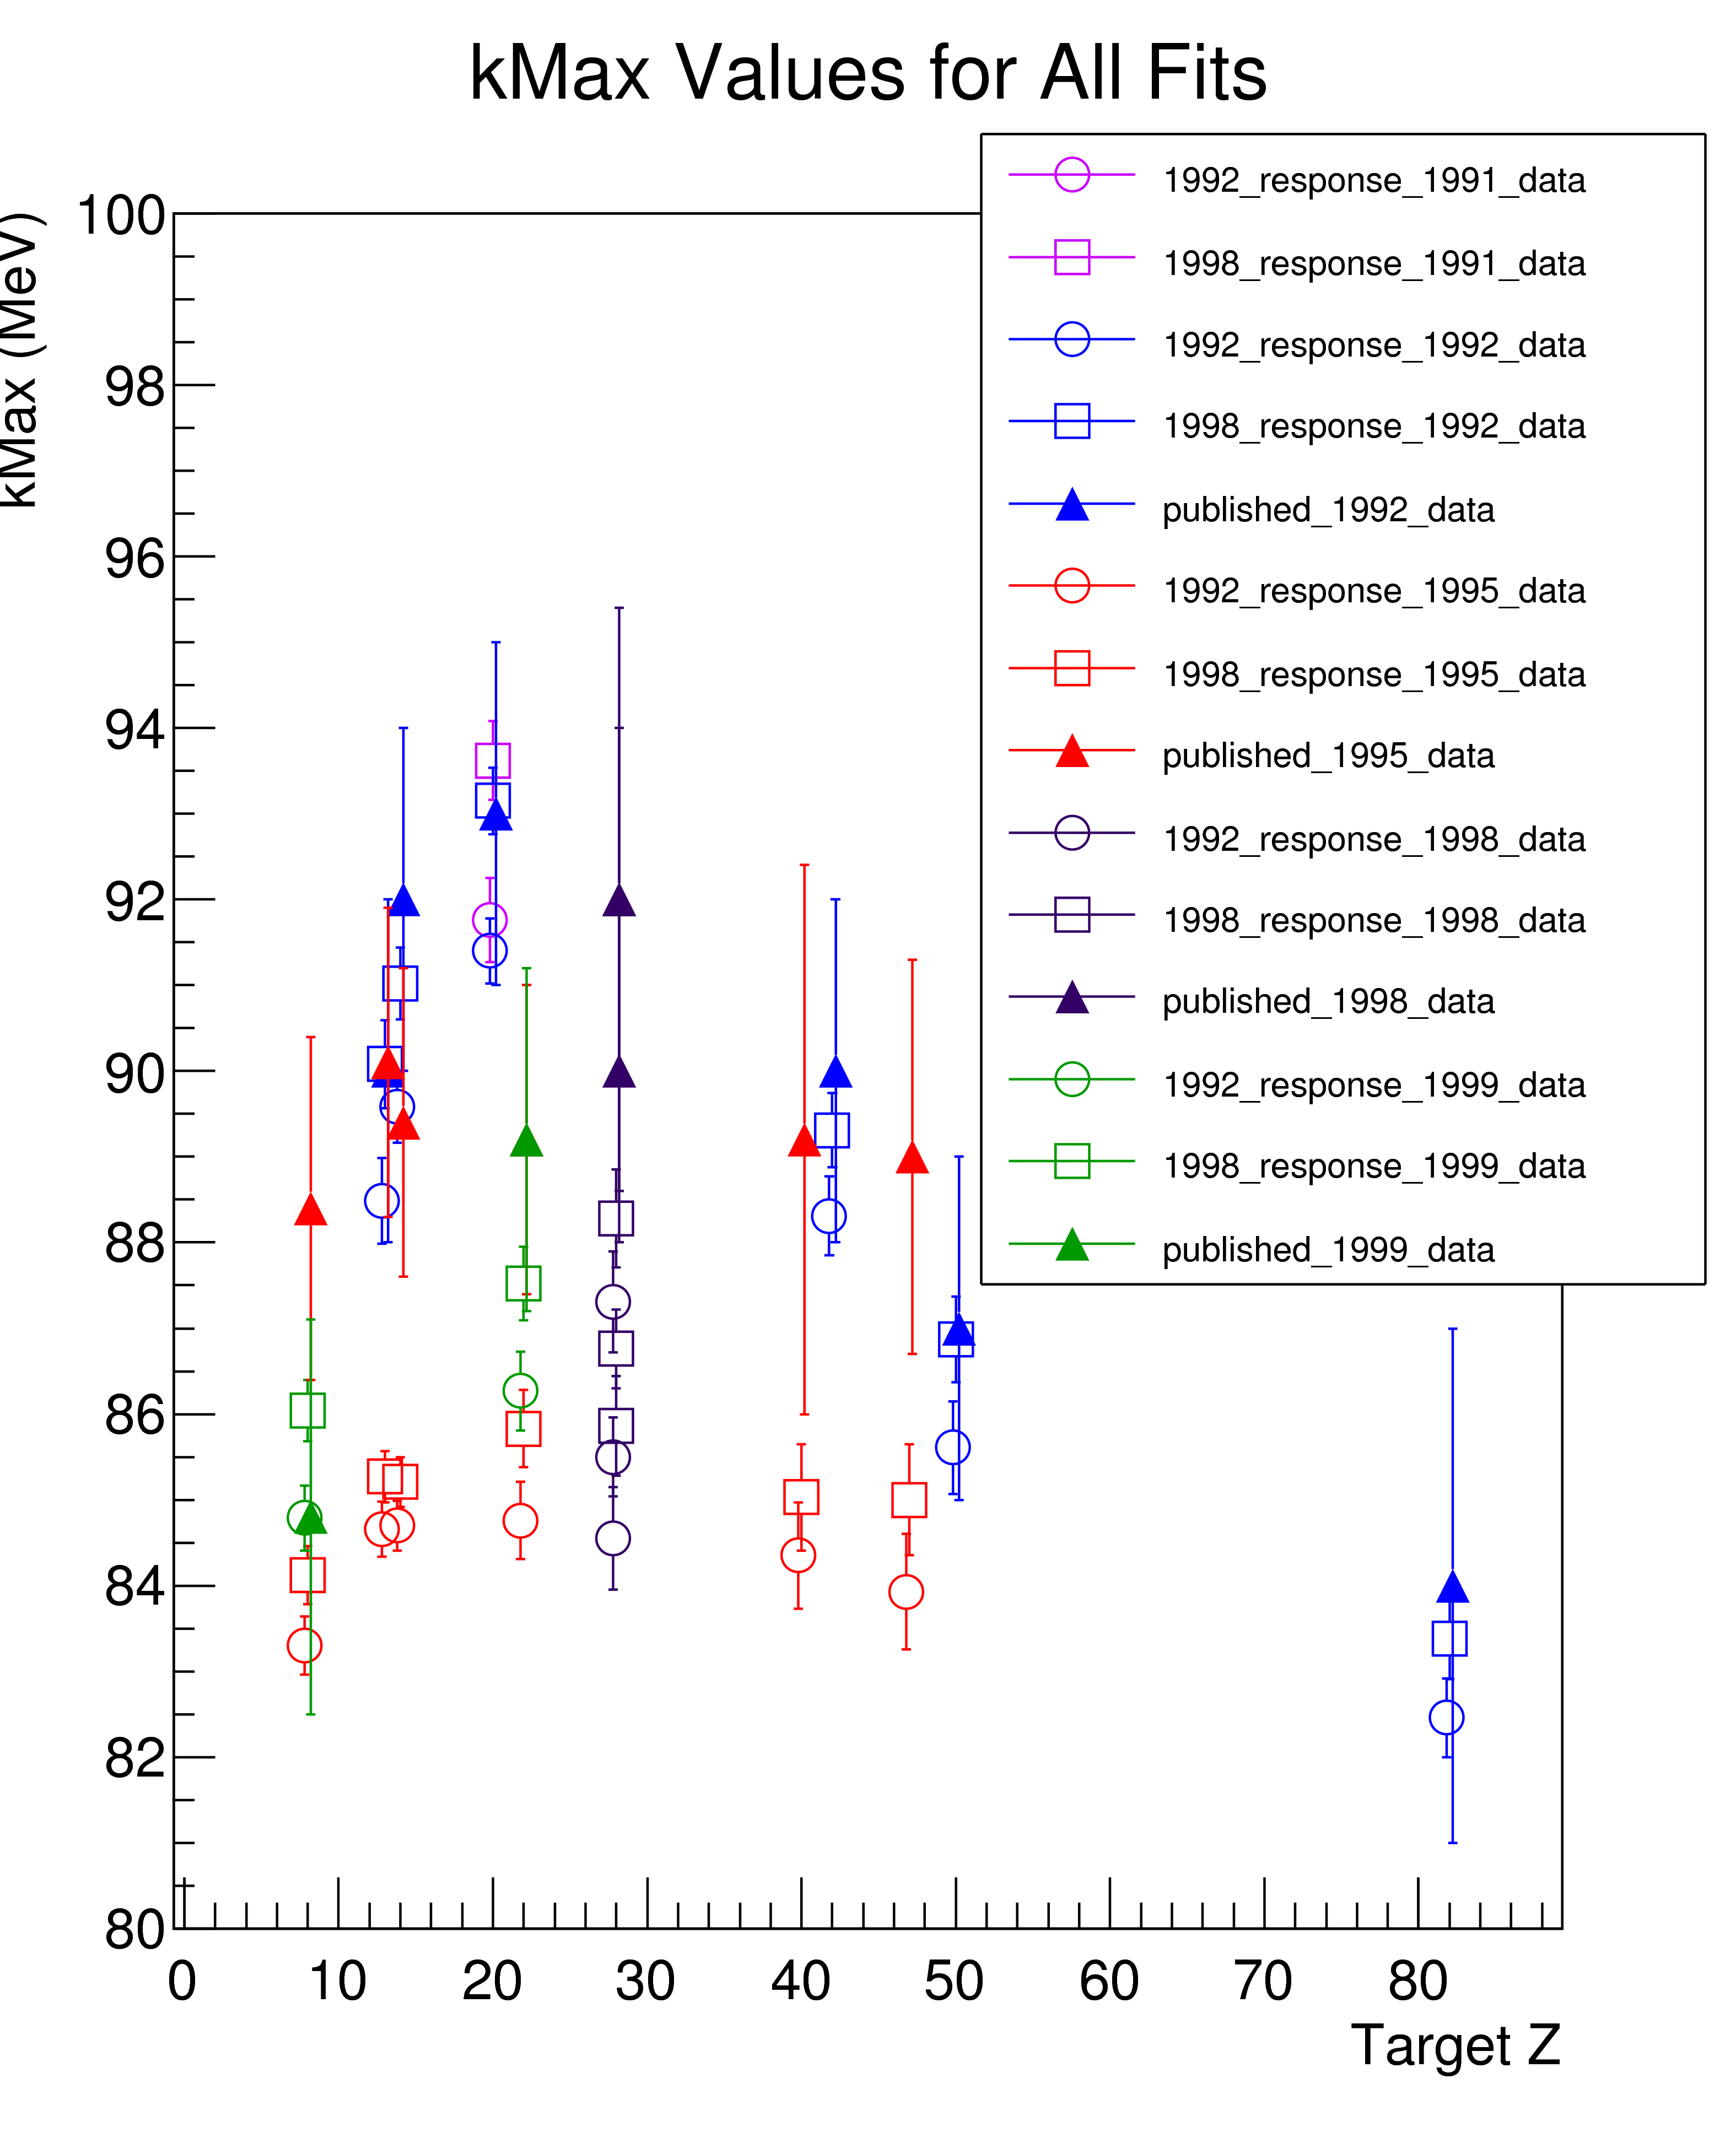
\includegraphics[width=0.48\linewidth]{figures/png/all_kMaxesChiSq_vs_target_z.png}
  }
  \hfill
  \subfloat[NLL Minimization Fit  \label{fig:NLL}]{%
  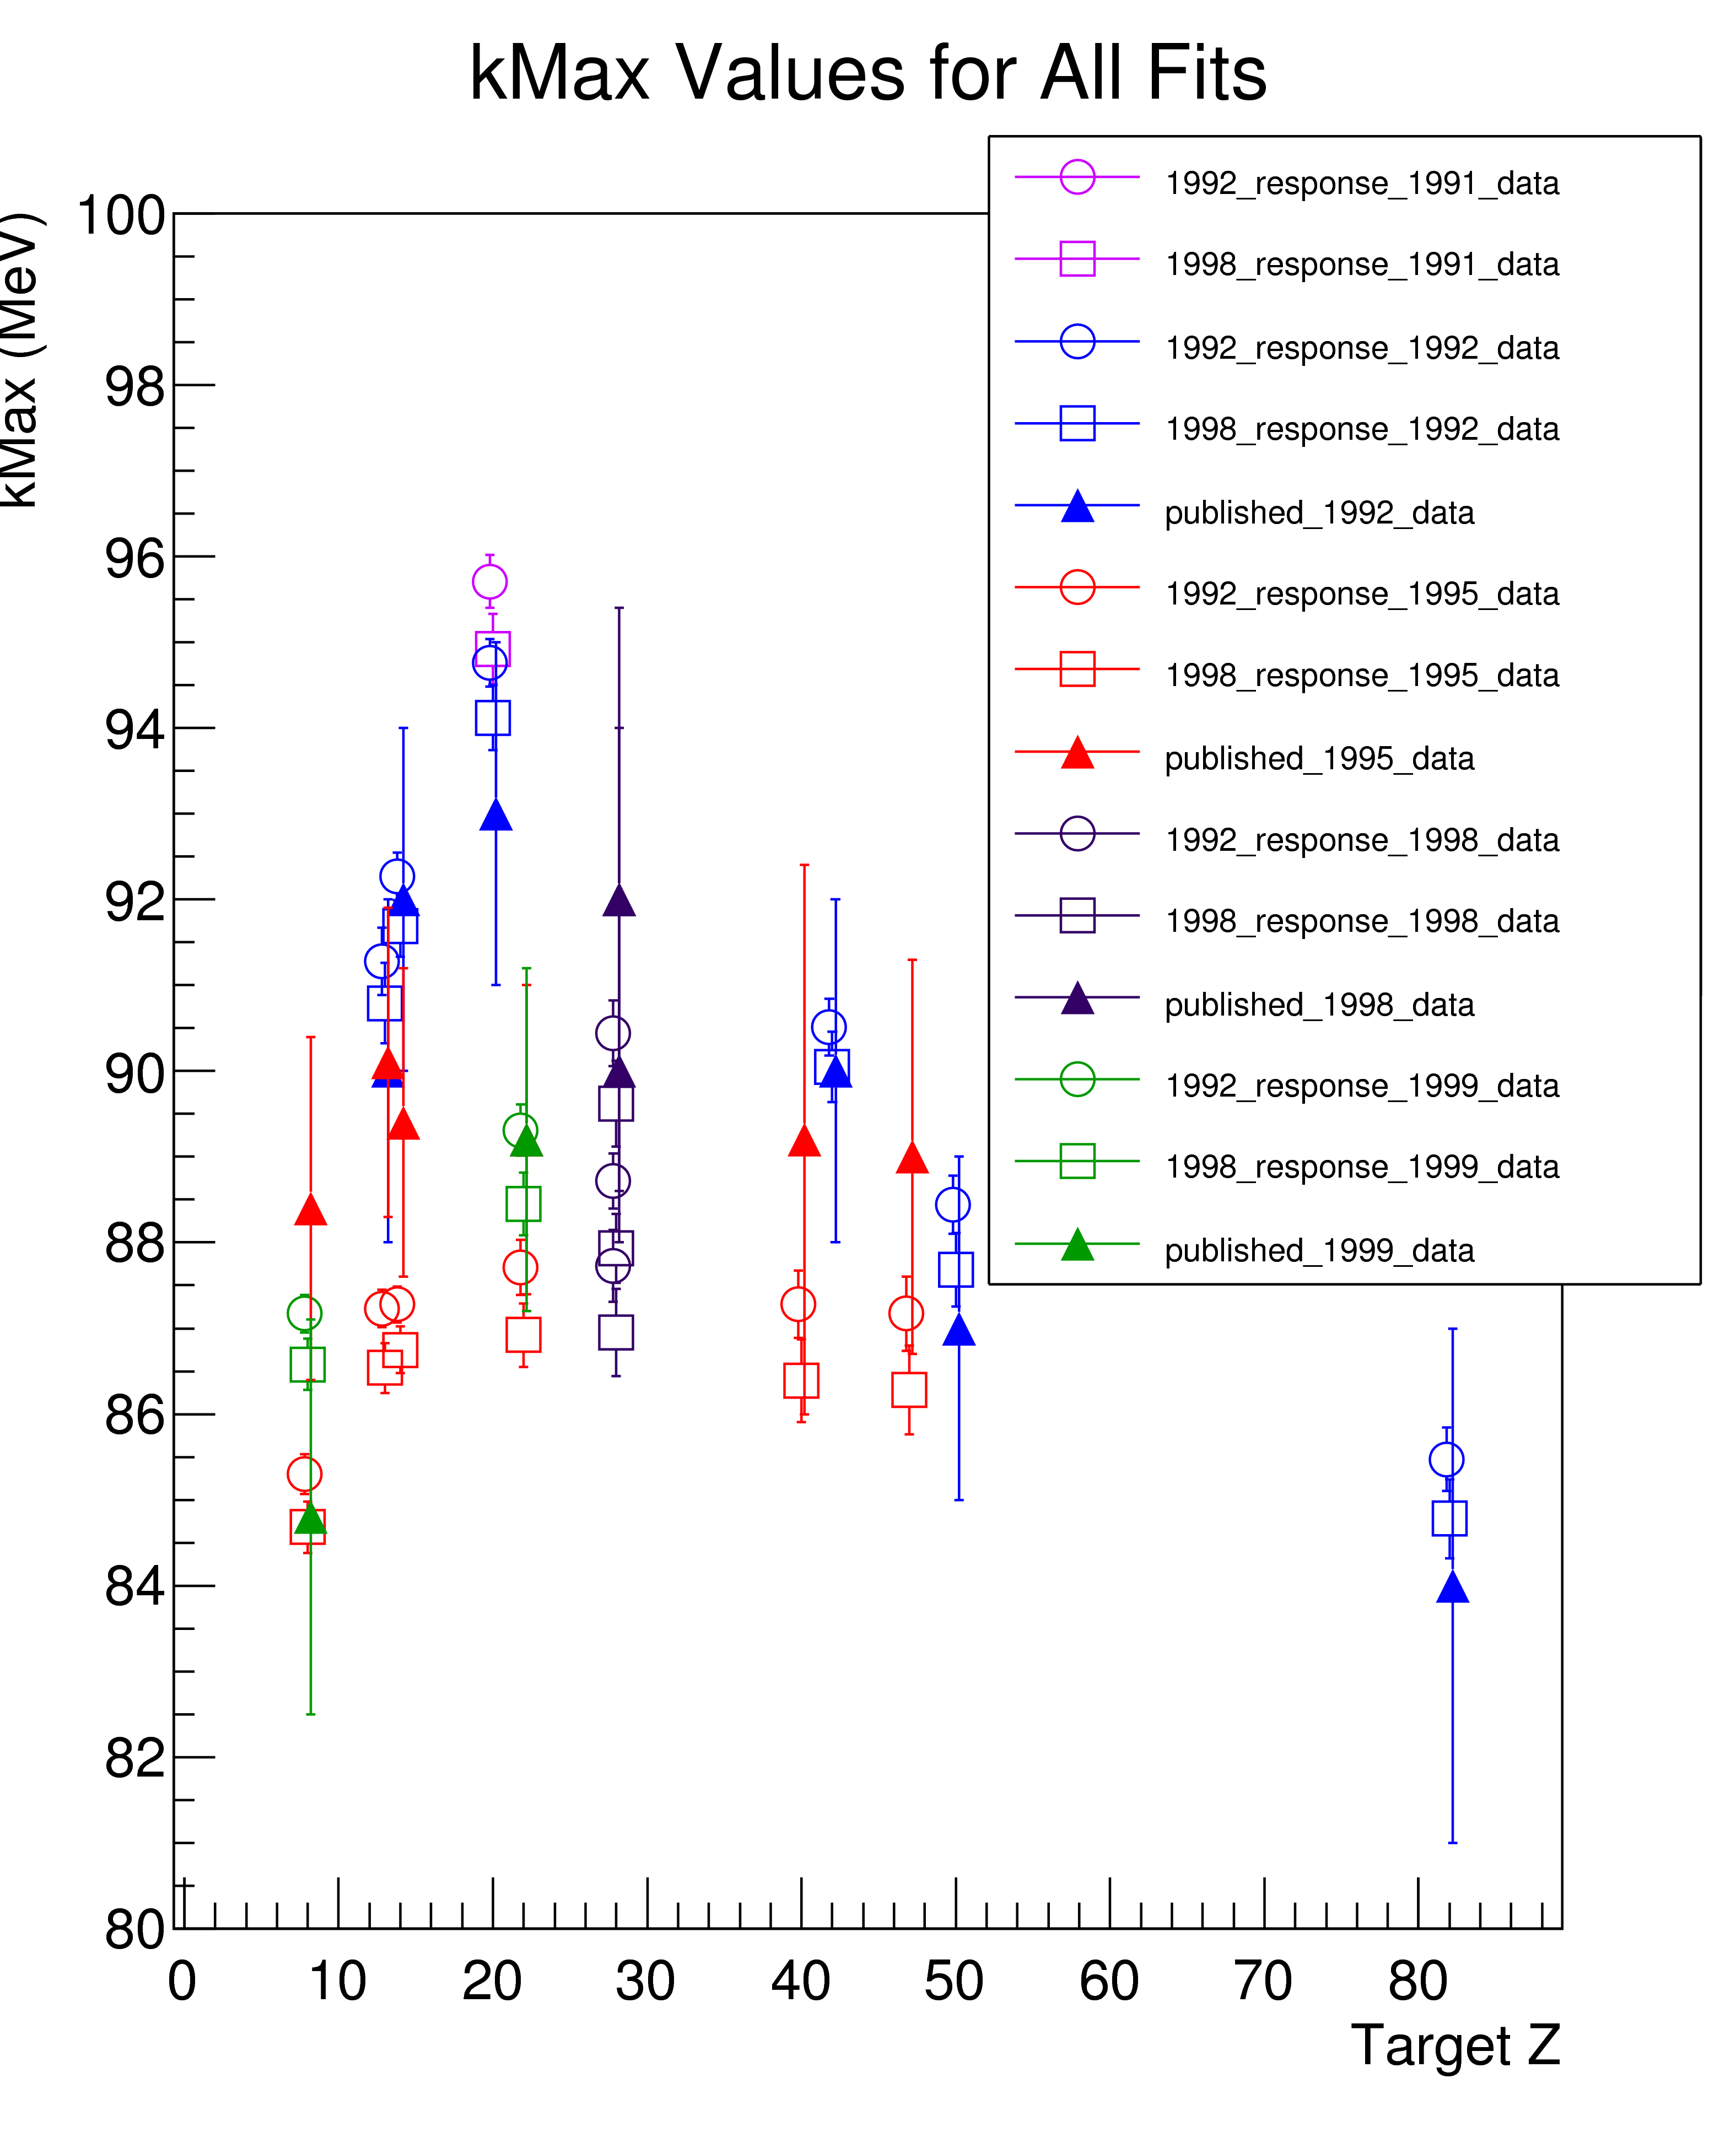
\includegraphics[width=0.48\linewidth]{figures/png/all_kMaxesNLL_vs_target_z.png}
  }
  \caption{Best fit end point value vs nuclear targets using (a) $\chi^2$ minimization and (b) NLL minimization.
    Triangular markers indicate the published values and uncertainty, circular markers indicate the results
    using the published 1992 response function, and square markers indicate the results using the published
    1998 response function. The 1992 response function data points are offset by -0.2 from their target z values
    and the published data points are offset by 0.2 from their target z values.
  }
\end{figure}
\begin{figure}[h]
  \centering
  \includegraphics[width=0.8\linewidth]{figures/png/chiSq_of_fits.png}
  \caption{Fit $\chi^2$ values for both response functions and both fitting methods. }
  \label{fig:ChiSqOfFits}
\end{figure}



%%%%%%%%%%%%%%%%%%%%%%%%%%%%%%%%%%%%%%%%%%%%%%%%%%%%%%%%%%%%%%%%%%%%%%%%%%%%%%

 %% Ca 1991 & & & 91.8 $\pm$ 0.5 &  3.7 (149.8 / 40) & 1992 & $\chi^2$ \\             
 %% Ca 1991 & & & 93.6 $\pm$ 0.5 &  1.4 (56.4 / 40) & 1998 & $\chi^2$ \\             
 %% Ca 1991 & & & 94.9 $\pm$ 0.4 & 1.4 ( 63.5 / 44) & 1998 & NNL \\                    
 %% Ca 1991 & & & 95.7 $\pm$ 0.3 & 4.9 ( 215.7 / 44) & 1992 & NNL \\                   


 %% Al 1992 & & & 88.5 $\pm$ 0.5 &  1.6 (56.0 / 34) & 1992 & $\chi^2$ \\             
 %% Al 1992 & & & 90.1 $\pm$ 0.5 &  1.2 (40.1 / 34) & 1998 & $\chi^2$ \\             

 %% Al 1992 & & & 91.3 $\pm$ 0.4 & 2.3 ( 100.9 / 43) & 1992 & NNL \\                   
 %% Al 1992 & & & 90.8 $\pm$ 0.5 & 1.5 ( 63.0 / 43) & 1998 & NNL \\                    

 %% Ca 1992 & & & 91.4 $\pm$ 0.4 &  2.6 (100.2 / 39) & 1992 & $\chi^2$ \\            
 %% Ca 1992 & & & 93.1 $\pm$ 0.4 &  1.4 (52.7 / 39) & 1998 & $\chi^2$ \\             

 %% Ca 1992 & & & 94.8 $\pm$ 0.3 & 4.6 ( 196.5 / 43) & 1992 & NNL \\                   
 %% Ca 1992 & & & 94.1 $\pm$ 0.4 & 1.7 ( 72.5 / 43) & 1998 & NNL \\                    

 %% Mo 1992 & & & 88.3 $\pm$ 0.5 &  1.6 (50.3 / 32) & 1992 & $\chi^2$ \\             
 %% Mo 1992 & & & 89.3 $\pm$ 0.4 &  0.8 (24.7 / 32) & 1998 & $\chi^2$ \\             

 %% Mo 1992 & & & 90.1 $\pm$ 0.4 & 0.7 ( 29.2 / 43) & 1998 & NNL \\                    
 %% Mo 1992 & & & 90.5 $\pm$ 0.3 & 1.6 ( 70.9 / 43) & 1992 & NNL \\                    

 %% Pb 1992 & & & 82.5 $\pm$ 0.5 &  1.3 (41.1 / 31) & 1992 & $\chi^2$ \\             
 %% Pb 1992 & & & 83.4 $\pm$ 0.5 &  0.6 (18.2 / 31) & 1998 & $\chi^2$ \\             

 %% Pb 1992 & & & 85.5 $\pm$ 0.4 & 2.1 ( 92.3 / 43) & 1992 & NNL \\                    
 %% Pb 1992 & & & 84.8 $\pm$ 0.5 & 0.7 ( 28.7 / 43) & 1998 & NNL \\                    

 %% Si 1992 & & & 89.6 $\pm$ 0.4 &  3.1 (102.9 / 33) & 1992 & $\chi^2$ \\            
 %% Si 1992 & & & 91.0 $\pm$ 0.4 &  1.3 (42.4 / 33) & 1998 & $\chi^2$ \\             

 %% Si 1992 & & & 92.3 $\pm$ 0.3 & 3.4 ( 147.7 / 43) & 1992 & NNL \\                   
 %% Si 1992 & & & 91.7 $\pm$ 0.4 & 1.2 ( 52.6 / 43) & 1998 & NNL \\                    

 %% Sn 1992 & & & 85.6 $\pm$ 0.5 &  2.4 (74.7 / 31) & 1992 & $\chi^2$ \\             
 %% Sn 1992 & & & 86.9 $\pm$ 0.5 &  0.7 (21.7 / 31) & 1998 & $\chi^2$ \\             

 %% Sn 1992 & & & 88.4 $\pm$ 0.3 & 2.5 ( 109.6 / 43) & 1992 & NNL \\                   
 %% Sn 1992 & & & 87.7 $\pm$ 0.4 & 0.6 ( 26.6 / 43) & 1998 & NNL \\                    


 %% Ag 1995 & & & 83.9 $\pm$ 0.7 &  2.0 (60.7 / 30) & 1992 & $\chi^2$ \\             
 %% Ag 1995 & & & 85.0 $\pm$ 0.7 &  1.0 (29.2 / 30) & 1998 & $\chi^2$ \\             

 %% Ag 1995 & & & 87.2 $\pm$ 0.4 & 2.2 ( 93.8 / 43) & 1992 & NNL \\
 %% Ag 1995 & & & 86.3 $\pm$ 0.5 & 0.8 ( 35.9 / 43) & 1998 & NNL \\                    

 %% Al 1995 & & & 84.7 $\pm$ 0.3 &  4.2 (134.9 / 32) & 1992 & $\chi^2$ \\            
 %% Al 1995 & & & 85.3 $\pm$ 0.3 &  1.3 (41.9 / 32) & 1998 & $\chi^2$ \\             

 %% Al 1995 & & & 87.2 $\pm$ 0.2 & 4.7 ( 203.1 / 43) & 1992 & NNL \\                   
 %% Al 1995 & & & 86.5 $\pm$ 0.3 & 1.3 ( 54.3 / 43) & 1998 & NNL \\                    

 %% O  1995 & & & 83.3 $\pm$ 0.3 &  4.5 (113.5 / 25) & 1992 & $\chi^2$ \\             
 %% O  1995 & & & 84.1 $\pm$ 0.3 &  1.3 (33.3 / 25) & 1998 & $\chi^2$ \\              

 %% O  1995 & & & 85.3 $\pm$ 0.2 & 3.6 ( 153.5 / 43) & 1992 & NNL \\                    
 %% O  1995 & & & 84.7 $\pm$ 0.3 & 1.1 ( 48.3 / 43) & 1998 & NNL \\                     

 %% Si 1995 & & & 84.7 $\pm$ 0.3 &  4.9 (151.5 / 31) & 1992 & $\chi^2$ \\            
 %% Si 1995 & & & 85.2 $\pm$ 0.3 &  2.3 (71.9 / 31) & 1998 & $\chi^2$ \\             

 %% Si 1995 & & & 87.3 $\pm$ 0.2 & 5.6 ( 241.5 / 43) & 1992 & NNL \\
 %% Si 1995 & & & 86.7 $\pm$ 0.3 & 2.4 ( 102.9 / 43) & 1998 & NNL \\                   

 %% Ti 1995 & & & 84.8 $\pm$ 0.5 &  3.6 (116.0 / 32) & 1992 & $\chi^2$ \\            
 %% Ti 1995 & & & 85.8 $\pm$ 0.4 &  1.5 (46.9 / 32) & 1998 & $\chi^2$ \\             

 %% Ti 1995 & & & 87.7 $\pm$ 0.3 & 3.9 ( 169.7 / 43) & 1992 & NNL \\
 %% Ti 1995 & & & 86.9 $\pm$ 0.4 & 1.3 ( 57.4 / 43) & 1998 & NNL \\                    

 %% Zr 1995 & & & 84.3 $\pm$ 0.6 &  2.9 (89.7 / 31) & 1992 & $\chi^2$ \\             
 %% Zr 1995 & & & 85.0 $\pm$ 0.6 &  1.6 (49.6 / 31) & 1998 & $\chi^2$ \\             

 %% Zr 1995 & & & 87.3 $\pm$ 0.4 & 2.9 ( 122.6 / 43) & 1992 & NNL \\
 %% Zr 1995 & & & 86.4 $\pm$ 0.5 & 1.4 ( 59.4 / 43) & 1998 & NNL \\                    


 %% Ni58 1998 & & & 87.3 $\pm$ 0.6 &  2.3 (73.7 / 32) & 1992 & $\chi^2$ \\
 %% Ni58 1998 & & & 88.3 $\pm$ 0.6 &  1.0 (32.7 / 32) & 1998 & $\chi^2$ \\

 %% Ni58 1998 & & & 90.4 $\pm$ 0.4 & 2.5 ( 107.2 / 43) & 1992 & NNL \\
 %% Ni58 1998 & & & 89.6 $\pm$ 0.5 & 0.9 ( 40.0 / 43) & 1998 & NNL \\

 %% Ni60 1998 & & & 85.5 $\pm$ 0.5 &  2.6 (84.4 / 33) & 1992 & $\chi^2$ \\
 %% Ni60 1998 & & & 86.8 $\pm$ 0.5 &  1.1 (36.4 / 33) & 1998 & $\chi^2$ \\

 %% Ni60 1998 & & & 88.7 $\pm$ 0.3 & 3.5 ( 151.1 / 43) & 1992 & NNL \\
 %% Ni60 1998 & & & 87.9 $\pm$ 0.4 & 1.1 ( 47.5 / 43) & 1998 & NNL \\

 %% Ni62 1998 & & & 84.6 $\pm$ 0.6 &  1.7 (51.1 / 30) & 1992 & $\chi^2$ \\
 %% Ni62 1998 & & & 85.9 $\pm$ 0.6 &  0.8 (25.1 / 30) & 1998 & $\chi^2$ \\

 %% Ni62 1998 & & & 87.7 $\pm$ 0.4 & 2.1 ( 89.2 / 43) & 1992 & NNL \\
 %% Ni62 1998 & & & 87.0 $\pm$ 0.5 & 0.7 ( 30.9 / 43) & 1998 & NNL \\


 %% O  1999 & & & 84.8 $\pm$ 0.4 &  5.6 (157.1 / 28) & 1992 & $\chi^2$ \\
 %% O  1999 & & & 86.0 $\pm$ 0.4 &  1.7 (46.7 / 28) & 1998 & $\chi^2$ \\

 %% O  1999 & & & 87.2 $\pm$ 0.2 & 5.0 ( 213.4 / 43) & 1992 & NNL \\
 %% O  1999 & & & 86.6 $\pm$ 0.3 & 2.2 ( 93.9 / 43) & 1998 & NNL \\

 %% Ti 1999 & & & 86.3 $\pm$ 0.5 &  3.7 (123.0 / 33) & 1992 & $\chi^2$ \\
 %% Ti 1999 & & & 87.5 $\pm$ 0.4 &  1.4 (47.7 / 33) & 1998 & $\chi^2$ \\

 %% Ti 1999 & & & 89.3 $\pm$ 0.3 & 4.2 ( 179.0 / 43) & 1992 & NNL \\
 %% Ti 1999 & & & 88.5 $\pm$ 0.4 & 1.2 ( 52.1 / 43) & 1998 & NNL \\


\subsection { Fits of the 1992 data }
\begin{table}[H]
  \begin{center}
    \begin{tabular}{|l||l|l|l|l|l|l|}
      \hline
      Dataset & Published $k_{Max}$ & $\chi^2 / DoF$ & Our $k_{Max}$ & $\chi^2 / DoF$  & Response & Fit \\
      \hhline{|=||=|=|=|=|=|=|}
       Al 1992   & 90.2 $\pm$ 2   & 1.1 & 88.5 $\pm$ 0.5 &  1.6 (56.0 / 34) & 1992 & $\chi^2$ \\  
                 &                &     & 90.1 $\pm$ 0.5 &  1.2 (40.1 / 34) & 1998 & $\chi^2$ \\  
                                                                             
                 &                &     & 91.3 $\pm$ 0.4 & 2.3 ( 100.9 / 43)& 1992 & NLL \\
                 &                &     & 90.8 $\pm$ 0.5 & 1.5 ( 63.0 / 43) & 1998 & NLL \\
       \hline                                                                
       Ca 1992   & 93   $\pm$ 2   & 1.6 & 91.4 $\pm$ 0.4 &  2.6 (100.2 / 39)& 1992 & $\chi^2$ \\  
                 &                &     & 93.1 $\pm$ 0.4 &  1.4 (52.7 / 39) & 1998 & $\chi^2$ \\  
                                                                             
                 &                &     & 94.8 $\pm$ 0.3 & 4.6 ( 196.5 / 43)& 1992 & NLL \\
                 &                &     & 94.1 $\pm$ 0.4 & 1.7 ( 72.5 / 43) & 1998 & NLL \\
      \hline                                                                 
       Mo 1992   & 90   $\pm$ 2   & 0.8 & 88.3 $\pm$ 0.5 &  1.6 (50.3 / 32) & 1992 & $\chi^2$ \\  
                 &                &     & 89.3 $\pm$ 0.4 &  0.8 (24.7 / 32) & 1998 & $\chi^2$ \\  
                                                                             
                 &                &     & 90.1 $\pm$ 0.4 & 0.7 ( 29.2 / 43) & 1992 & NLL \\
                 &                &     & 90.5 $\pm$ 0.3 & 1.6 ( 70.9 / 43) & 1998 & NLL \\
      \hline                                                                 
       Pb 1992   & 84   $\pm$ 3   & 0.9 & 82.5 $\pm$ 0.5 &  1.3 (41.1 / 31) & 1992 & $\chi^2$ \\  
                 &                &     & 83.4 $\pm$ 0.5 &  0.6 (18.2 / 31) & 1998 & $\chi^2$ \\  
                                                                             
                 &                &     & 85.5 $\pm$ 0.4 & 2.1 ( 92.3 / 43) & 1992 & NLL \\
                 &                &     & 84.8 $\pm$ 0.5 & 0.7 ( 28.7 / 43) & 1998 & NLL \\
      \hline                                                                 
       Si 1992   & 92.2 $\pm$ 2   & 1.7 & 89.6 $\pm$ 0.4 &  3.1 (102.9 / 33)& 1992 & $\chi^2$ \\  
                 &                &     & 91.0 $\pm$ 0.4 &  1.3 (42.4 / 33) & 1998 & $\chi^2$ \\  
                                                                             
                 &                &     & 92.3 $\pm$ 0.3 & 3.4 ( 147.7 / 43)& 1992 & NLL \\
                 &                &     & 91.7 $\pm$ 0.4 & 1.2 ( 52.6 / 43) & 1998 & NLL \\
      \hline                                                                 
       Sn 1992   & 87   $\pm$ 2   & 1.1 & 85.6 $\pm$ 0.5 &  2.4 (74.7 / 31) & 1992 & $\chi^2$ \\  
                 &                &     & 86.9 $\pm$ 0.5 &  0.7 (21.7 / 31) & 1998 & $\chi^2$ \\  
                                                                             
                 &                &     & 88.4 $\pm$ 0.3 & 2.5 ( 109.6 / 43) & 1992 & NLL \\
                 &                &     & 87.7 $\pm$ 0.4 & 0.6 ( 26.6 / 43) & 1998 & NLL \\
      \hline                           
    \end{tabular}
  \end{center}
  \caption{The fit results.}
  \label{table:fits1992}
\end{table}

%%%%%%%%%%%%%%%%%%%%%%%%%%%%%%%%%%%%%%%%%%%%%%%%%%%%%%%%%%%%%%%%%%%%%%%%%%%%%%
\subsection { Fits of the 1995 data }

\begin{table}[H]
  \begin{center}
    \begin{tabular}{|l||l|l|l|l|l|l|}
      \hline
      Dataset & Published $k_{Max}$ & $\chi^2 / DoF$ & Our $k_{Max}$ & $\chi^2 / DoF$  & Response & Fit \\
      \hhline{|=||=|=|=|=|=|=|}
       Ag 1995   & 89.0 $\pm$ 3.2 & 1.2 &83.9 $\pm$ 0.7 &  2.0 (60.7 / 30)  & 1992 & $\chi^2$ \\  
                 &                &     &85.0 $\pm$ 0.7 &  1.0 (29.2 / 30)  & 1998 & $\chi^2$ \\  
                                                                             
                &                &     & 87.2 $\pm$ 0.4 & 2.2 ( 93.8 / 43) & 1992 & NLL \\
                &                &     & 86.3 $\pm$ 0.5 & 0.8 ( 35.9 / 43) & 1998 & NLL \\      
      \hline                                                                
       Al 1995   & 90.1 $\pm$ 1.8 & 1.5 &84.7 $\pm$ 0.3 &  4.2 (134.9 / 32) & 1992 & $\chi^2$ \\  
                 &                &     &85.3 $\pm$ 0.3 &  1.3 (41.9 / 32)  & 1998 & $\chi^2$ \\  
                                                                            
                &                &     & 87.2 $\pm$ 0.2 & 4.7 ( 203.1 / 43) & 1992 & NLL \\
                &                &     & 86.5 $\pm$ 0.3 & 1.3 ( 54.3 / 43) & 1998 & NLL \\
      \hline                                                                
       O 1995    & 88.4 $\pm$ 2.3 & 2.1 &83.3 $\pm$ 0.3 &  4.5 (113.5 / 25) & 1992 & $\chi^2$ \\  
                 &                &     &84.1 $\pm$ 0.3 &  1.3 (33.3 / 25)  & 1998 & $\chi^2$ \\  
                                                                            
                &                &     & 85.3 $\pm$ 0.2 & 3.6 ( 153.5 / 43)& 1992 & NLL\\
                &                &     & 84.7 $\pm$ 0.3 & 1.1 ( 48.3 / 43) & 1998 & NLL\\
      \hline                                                                     
       Si 1995   & 89.4 $\pm$ 1.8 & 2.7 &84.7 $\pm$ 0.3 &  4.9 (151.5 / 31) & 1992 & $\chi^2$ \\  
                 &                &     &85.2 $\pm$ 0.3 &  2.3 (71.9 / 31)  & 1998 & $\chi^2$ \\  
                                                                             
                &                &     & 87.3 $\pm$ 0.2 & 5.6 ( 241.5 / 43) & 1992 & NLL \\
                &                &     & 86.7 $\pm$ 0.3 & 2.4 ( 102.9 / 43)& 1998 & NLL \\
      \hline                                                                
       Ti 1995   & 89.2 $\pm$ 2.0 & 1.9 &84.8 $\pm$ 0.5 &  3.6 (116.0 / 32) & 1992 & $\chi^2$ \\  
                 &                &     &85.8 $\pm$ 0.4 &  1.5 (46.9 / 32)  & 1998 & $\chi^2$ \\  
                                                                            
                &                &     & 87.7 $\pm$ 0.3 & 3.9 ( 169.7 / 43) & 1992 & NLL \\
                &                &     & 86.9 $\pm$ 0.4 & 1.3 ( 57.4 / 43) & 1998 & NLL \\
      \hline                                                                
       Zr 1995   & 89.2 $\pm$ 3.4 & 1.2 &84.3 $\pm$ 0.6 &  2.9 (89.7 / 31)  & 1992 & $\chi^2$ \\  
                 &                &     &85.0 $\pm$ 0.6 &  1.6 (49.6 / 31)  & 1998 & $\chi^2$ \\  
                                                                            
                &                &     & 87.3 $\pm$ 0.4 & 2.9 ( 122.6 / 43) & 1992 & NLL \\
                &                &     & 86.4 $\pm$ 0.5 & 1.4 ( 59.4 / 43) & 1998 & NLL \\
      \hline
                                                                                
    \end{tabular}
  \end{center}
  \caption{The fit results.}
  \label{table:fits1995}
\end{table}


%%%%%%%%%%%%%%%%%%%%%%%%%%%%%%%%%%%%%%%%%%%%%%%%%%%%%%%%%%%%%%%%%%%%%%%%%%%%%%
\subsection { Fits of the 1998 data }
\begin{table}[H]
  \begin{center}
    \begin{tabular}{|l||l|l|l|l|l|l|}
      \hline
      Dataset & Published $k_{Max}$ & $\chi^2 / DoF$ & Our $k_{Max}$ & $\chi^2 / DoF$  & Response & Fit \\
      \hhline{|=||=|=|=|=|=|=|}
       Ni58 1998 & 92   $\pm$ 2   & 1.8 & 87.3 $\pm$ 0.6 &  2.3 (73.7 / 32) & 1992 & $\chi^2$ \\  
                 &                &     & 88.3 $\pm$ 0.6 &  1.0 (32.7 / 32) & 1998 & $\chi^2$ \\  
                                                                             
                &                 &     & 90.4 $\pm$ 0.4 & 2.5 ( 107.2 / 43) & 1992 & NLL \\
                &                 &     & 89.6 $\pm$ 0.5 & 0.9 ( 40.0 / 43) & 1998 & NLL \\
      \hline                                                                 
       Ni60 1998 & 92   $\pm$ 2   & 2.0 & 85.5 $\pm$ 0.5 &  2.6 (84.4 / 33) & 1992 & $\chi^2$ \\  
                 &                &     & 86.8 $\pm$ 0.5 &  1.1 (36.4 / 33) & 1998 & $\chi^2$ \\  
                                                                             
                &                 &     & 88.7 $\pm$ 0.3 & 3.5 ( 151.1 / 43) & 1992 & NLL \\
                &                 &     & 87.9 $\pm$ 0.4 & 1.1 ( 47.5 / 43) & 1998 & NLL \\
      \hline                                                                 
       Ni62 1998 & 90   $\pm$ 2   & 1.3 & 84.6 $\pm$ 0.6 &  1.7 (51.1 / 30) & 1992 & $\chi^2$ \\  
                 &                &     & 85.9 $\pm$ 0.6 &  0.8 (25.1 / 30) & 1998 & $\chi^2$ \\  
                                                                             
                &                 &     & 87.7 $\pm$ 0.4 & 2.1 ( 89.2 / 43) & 1992 & NLL \\
                &                 &     & 87.0 $\pm$ 0.5 & 0.7 ( 30.9 / 43) & 1998 & NLL \\
      \hline                           
    \end{tabular}
  \end{center}
  \caption{The fit results.}
  \label{table:fits1998}
\end{table}

%%%%%%%%%%%%%%%%%%%%%%%%%%%%%%%%%%%%%%%%%%%%%%%%%%%%%%%%%%%%%%%%%%%%%%%%%%%%%%
\subsection { Fits of the 1999 data }

\begin{table}[H]
  \begin{center}
    \begin{tabular}{|l||l|l|l|l|l|l|}
      \hline
      Dataset & Published $k_{Max}$ & $\chi^2 / DoF$ & Our $k_{Max}$ & $\chi^2 / DoF$  & Response & Fit \\
      \hhline{|=||=|=|=|=|=|=|}
       O 1999    & 88.4 $\pm$ 2.3 & 2.1 & 84.8 $\pm$ 0.4 &  5.6 (157.1 / 28)& 1992 & $\chi^2$ \\  
                 &                &     & 86.0 $\pm$ 0.4 &  1.7 (46.7 / 28) & 1998 & $\chi^2$ \\  
                                                                             
                 &                &     & 87.2 $\pm$ 0.2 & 5.0 ( 213.4 / 43)& 1992 & NLL\\
                 &                &     & 86.6 $\pm$ 0.3 & 2.2 ( 93.9 / 43) & 1998 & NLL\\
      \hline                                                                 
       Ti 1999   & 89.2 $\pm$ 2.0 & 1.9 & 86.3 $\pm$ 0.5 &  3.7 (123.0 / 33)& 1992 & $\chi^2$ \\  
                 &                &     & 87.5 $\pm$ 0.4 &  1.4 (47.7 / 33) & 1998 & $\chi^2$ \\  
                                                                             
                 &                &     & 89.3 $\pm$ 0.3 & 4.2 ( 179.0 / 43) & 1992 & NLL \\
                 &                &     & 88.5 $\pm$ 0.4 & 1.2 ( 52.1 / 43) & 1998 & NLL \\
      \hline                           
    \end{tabular}
  \end{center}
  \caption{The fit results.}
  \label{table:fits1999}
\end{table}

\begin{figure}[h]
  \centering
  \includegraphics[width=\linewidth]{figures/png/compare_fit_results.png}
  \caption{Plot of the difference between the end point values found using $\chi^2$ and
    NLL minimization with and without a restricted range using the 1998 response function.}
  \label{fig:compareFits}
\end{figure}

\begin{figure}[h]
  \centering
  \includegraphics[width=\linewidth]{figures/png/compare_fit_results_unrestrictedOnly.png}
  \caption{Plot of the difference between the end point values found using $\chi^2$ and
    NLL minimization using the 1998 response function.}
  \label{fig:compareFits}
\end{figure}


